\documentclass[11pt, a4paper]{article}

\usepackage[affil-it]{authblk}
\usepackage{etoolbox}
\usepackage{lmodern}
\usepackage{titlesec}
\usepackage{float}
\usepackage{amsfonts}
\usepackage{hyperref}
\usepackage{listings}
\usepackage{color}
\usepackage{graphicx}
\usepackage{subcaption}
\usepackage{amsmath}
\usepackage{relsize}

\makeatletter
\patchcmd{\@maketitle}{\LARGE \@title}{\fontsize{20}{19.2}\selectfont\@title}{}{}
\makeatother

\renewcommand\Authfont{\fontsize{16}{14.4}\selectfont}
\renewcommand\Affilfont{\fontsize{12}{10.8}\itshape}

\title{\textbf{AE 706: Assignment 1}}
\author{Pavan R Hebbar - 130010046}

\definecolor{codegreen}{rgb}{0,0.6,0}
\definecolor{codegray}{rgb}{0.5,0.5,0.5}
\definecolor{codepurple}{rgb}{0.58,0,0.82}
\definecolor{backcolour}{rgb}{0.95,0.95,0.92}
 
\lstdefinestyle{mystyle}{
    backgroundcolor=\color{backcolour},   
    commentstyle=\color{codegreen},
    keywordstyle=\color{magenta},
    numberstyle=\tiny\color{codegray},
    stringstyle=\color{codepurple},
    basicstyle=\footnotesize,
    breakatwhitespace=false,         
    breaklines=true,                 
    captionpos=b,                    
    keepspaces=true,                 
    numbers=left,                    
    numbersep=5pt,                  
    showspaces=false,                
    showstringspaces=false,
    showtabs=false,                  
    tabsize=2
}
\lstset{style=mystyle}

\begin{document}
\maketitle
\newpage
\tableofcontents
\newpage
\section{Introduction:}
This assignment deals with the different methods used to solve the Laplace equation and their convergence rates. We particularly
discuss the Jacobi, Gauss Siedel and the Successive Over relaxation methods and compare their convergence rates.

In Question 1, we compute and plot the convergence rates of Jacobi and Gauss Siedel schemes for different grid
sizes. In Question 2,3, 4 we hunt for the optimum value of $w$ in the SOR scheme to minimize the error after fixed 
number of iterations for $N=41$.
In Question 5, 6 we find the optimum value $w$ for N=41. In Question 7 we compare all the three schemes for $N = 101$
Throughout the assignment we use the definition of error as :
\begin{equation}
 err = \frac{\sqrt{\Sigma_{i,j}(\phi_{i,j}^{n+1} - \phi_{i,j}^{n})^2}}{N}
\end{equation}
All plots are plotted in semilog form

\section{Question 1:}
\label{Question1}

In this question we plot the convergence rate of Jacobi and Gauss Siedel methods for $N = 11, 21, 41, 101$. To achieve this we
plot the error versus the iteration no. and repeat the process until $err = 2*machineepsilon$.
For this purpose we defined functions to calculate the successive $\phi$ from the previous $\phi$. The codes for one jacobi and
Gauss Siedel iterations are mentioned below
\begin{lstlisting}[language = Python, caption = Function to perform 1 iteration of Jacobi]
def jacobi_step(phi_in):
    phi_new = phi_in.copy()
    phi_new[1:-1, 1:-1] = 0.25*(phi_in[0:-2, 1:-1] + phi_in[2:,1:-1] + phi_in[1:-1,0:-2] + phi_in[1:-1,2:])
    return phi_new

\end{lstlisting}
\begin{lstlisting}[language = Python, caption = Function to perform 1 iteration of Gauss Siedel]
 def gs_step(phi_in):
    phi_next = phi_in.copy()
    N = phi_in.shape[0]
    for i in range(1, N-1):
        for j in range(1, N-1):
            phi_next[i, j] = (phi_in[i+1, j] + phi_in[i, j+1] + phi_next[i-1, j] + phi_next[i, j-1])*0.25

    return phi_next
\end{lstlisting}

We also write a general function to solve the Laplace equation numerically:
\begin{lstlisting}[language = Python, caption = Function to solve Laplace equation by given method]
def solve_lap(phi_in, method, nmax):
    N = phi_in.shape[0]
    error_arr = np.array([])
    niter = 0
    error = 1.0
    while(error >= 2*EPSILON and niter <= nmax):
        phi_new = method(phi_in.copy())
        error = error_q(phi_new, phi_in)
        phi_in = phi_new.copy()
        error_arr = np.append(error_arr.copy(), error)
        niter += 1
    return error_arr
\end{lstlisting}

On running the code we get the following graphs
\begin{figure}[H]
 \centering
 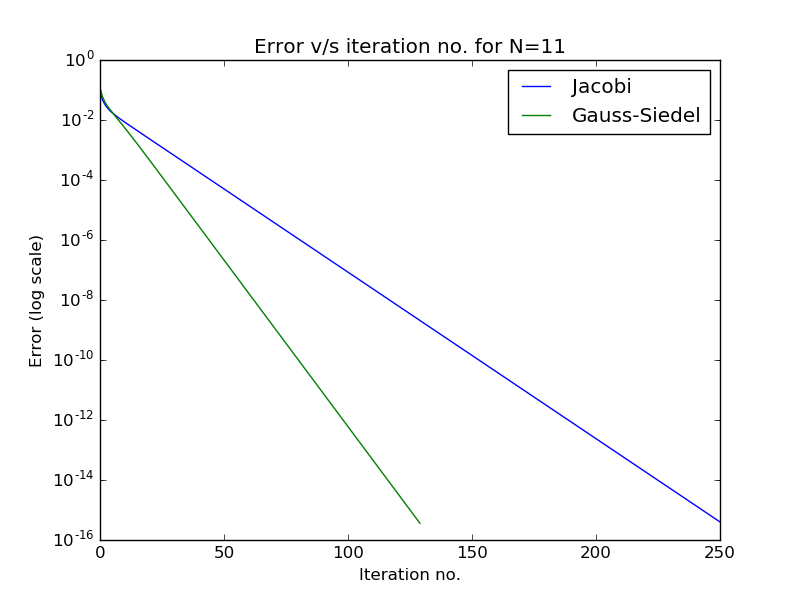
\includegraphics[width = 0.8\textwidth]{N_11.png}
 \caption{Jacobi and Gauss Siedel errors for N = 11}
\end{figure}

\begin{figure}[H]
 \centering
 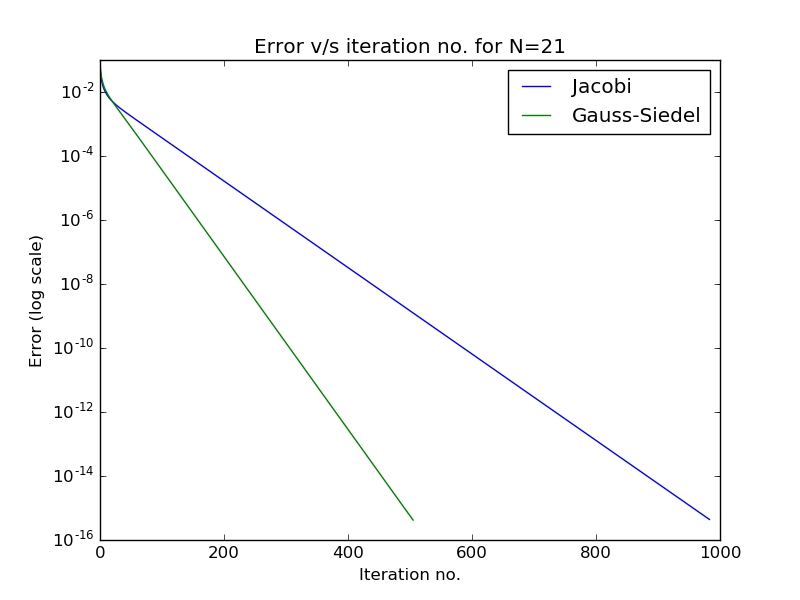
\includegraphics[width = 0.8\textwidth]{N_21.png}
 \caption{Jacobi and Gauss Siedel errors for N = 21}
\end{figure}

\begin{figure}[H]
 \centering
 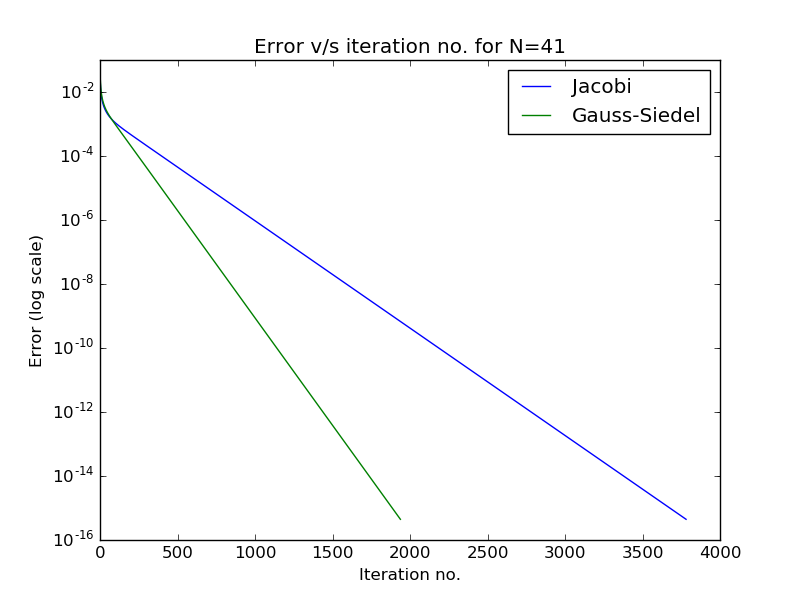
\includegraphics[width = 0.8\textwidth]{N_41.png}
 \caption{Jacobi and Gauss Siedel errors for N = 41}
\end{figure}

\begin{figure}[H]
 \centering
 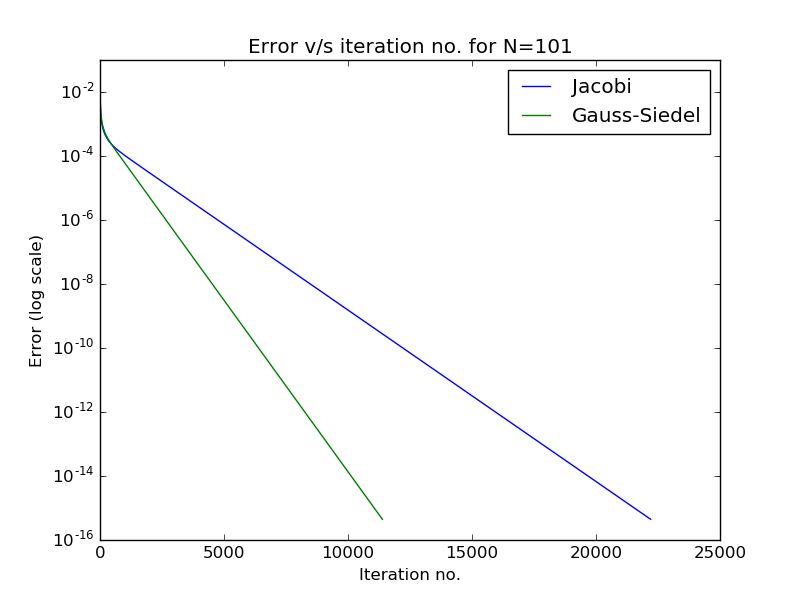
\includegraphics[width = 0.8\textwidth]{N_101.png}
 \caption{Jacobi and Gauss Siedel errors for N = 101}
\end{figure}

From the graphs, it can be seen that the Gauss Siedel method converges about twice as fast as Jacobi method. Also we see that
the convergence of both the schemes decreases the the grid size decreases. Thus we can achieve fast convergence from coarse 
gridding.

Below are the plots of the residue plotted with the iteration number:
\begin{figure}[H]
 \centering
 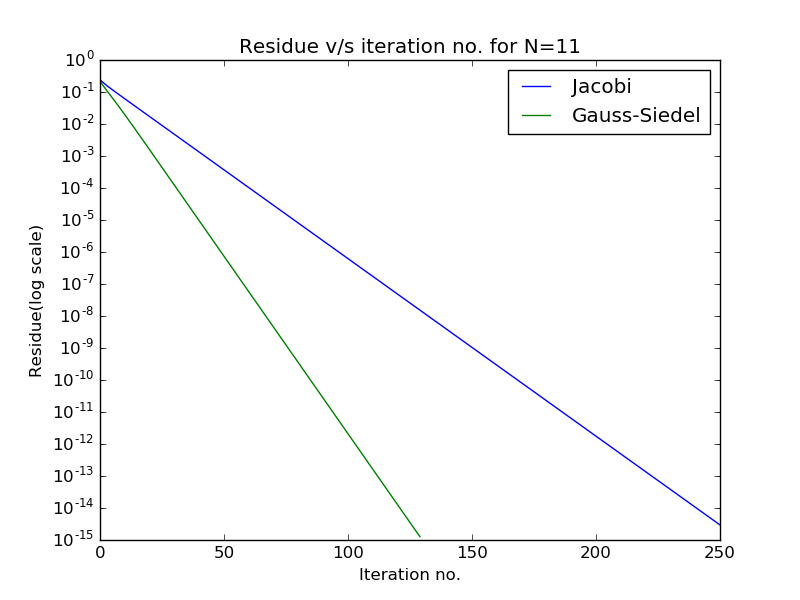
\includegraphics[width = 0.8\textwidth]{N_11_1.png}
 \caption{Jacobi and Gauss Siedel residue for N = 11}
\end{figure}

\begin{figure}[H]
 \centering
 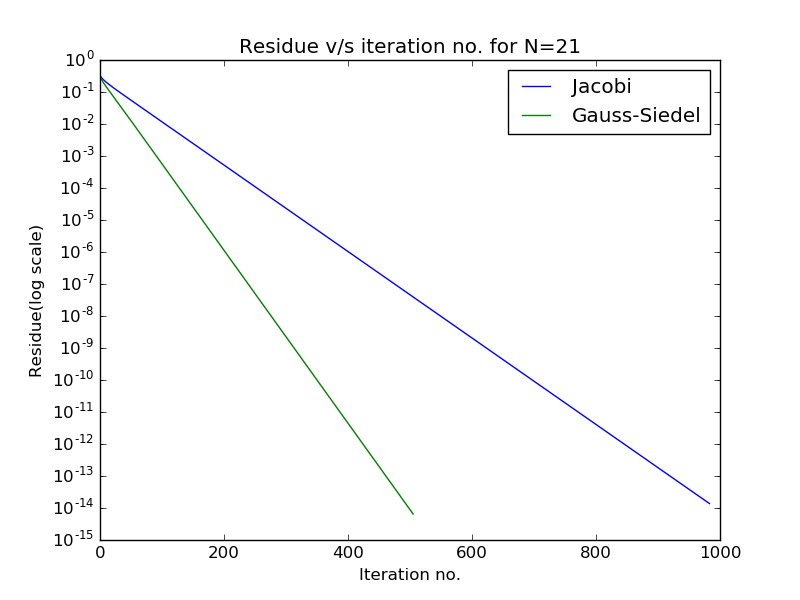
\includegraphics[width = 0.8\textwidth]{N_21_1.png}
 \caption{Jacobi and Gauss Siedel residue for N = 21}
\end{figure}

\begin{figure}[H]
 \centering
 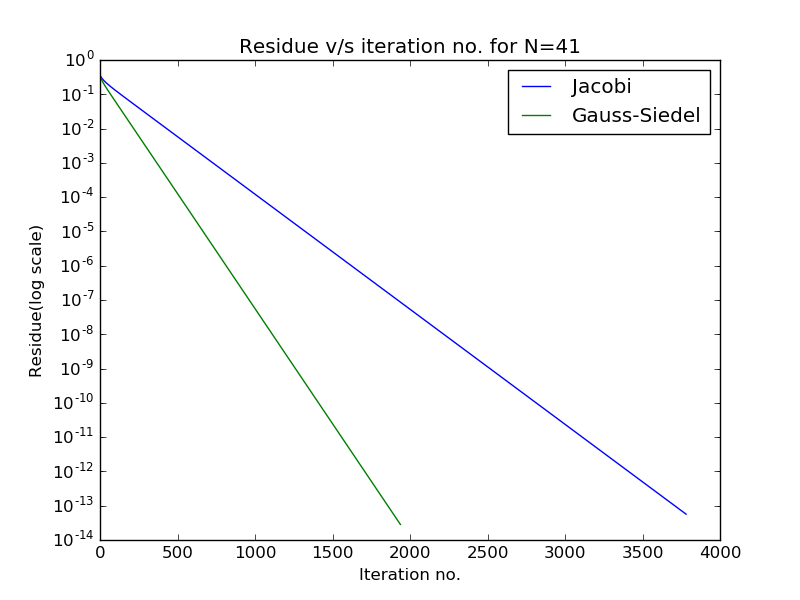
\includegraphics[width = 0.8\textwidth]{N_41_1.png}
 \caption{Jacobi and Gauss Siedel residue for N = 41}
\end{figure}

\begin{figure}[H]
 \centering
 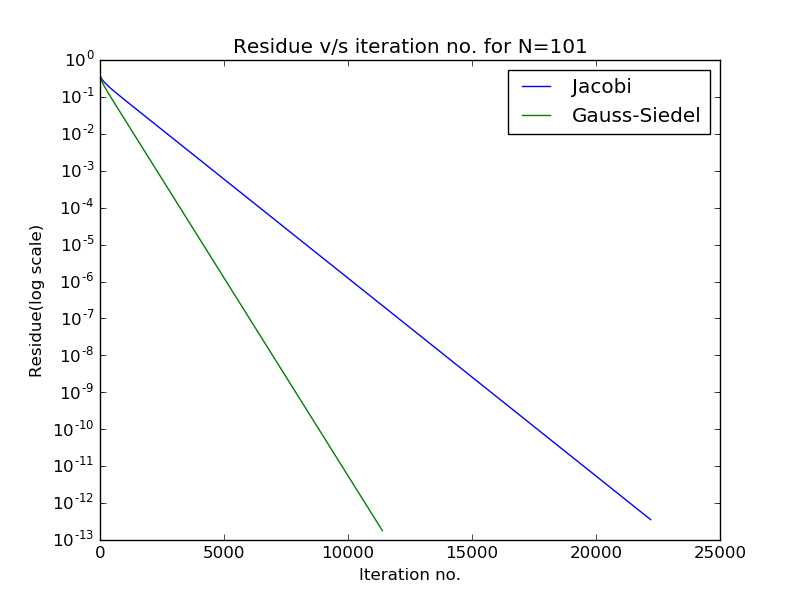
\includegraphics[width = 0.8\textwidth]{N_101_1.png}
 \caption{Jacobi and Gauss Siedel residue for N = 101}
\end{figure}



\section{Question 2:}
Here we fix our grid size with $N = 41$ and the number of iterations to $20$. We then vary the $w$ from $0.1$ to $2.0$ with
steps of $0.1$ to compute the $w$ which gives minimum error.
For this purpose we write a function for the SOR scheme when the $w$ is specified:
\begin{lstlisting}[language = Python, caption = Function to solve Laplace equation by SOR scheme]
def sor(phi_in, nmax, w):
    N = phi_in.shape[0]
    niter = 0
    error = 1.0
    error_sor = np.array([])
    phi_new = phi_in.copy()
    while(error >= 2*EPSILON and niter <= nmax):
        phi_old = phi_new.copy()
        for i in range (1, N-1):
            for j in range (1, N-1):
                phi_new[i,j] = (1 - w)*phi_old[i,j] + w*0.25*(phi_new[i+1,j]+phi_new[i-1,j]+phi_new[i,j+1]+phi_new[i,j-1])
        error = error_q(phi_new, phi_old)
        error_sor = np.append(error_sor.copy(), error)
        niter += 1
    return error_sor
\end{lstlisting}
We then write a generalized function to compute the error after fixed number of iterations for a range of $w$.
\begin{lstlisting}[language = Python, caption = Function to solve Laplace equation by SOR scheme for range of w]
def sor_range(phi_in, nmax, wmin, wmax, wstep): 
    N = phi_in.shape[0]
    w = np.arange(wmin, wmax, wstep)
    error = np.zeros(len(w))
    niter = np.zeros(len(w))
    for i in range(len(w)):
        err = sor(phi_in, nmax, w[i])
        error[i] = err[-1]
        niter[i] = err.shape[0]
    wminerr = w[np.argmin(error)]
    return error, niter, wminerr
\end{lstlisting}

This functions yields the final error value after the given number of iterations, the number of iterations performed and the
optimum w. We get the following plot of error vs w for $N=41$ and $20$ iterations.


\begin{figure}[H]
 \centering
 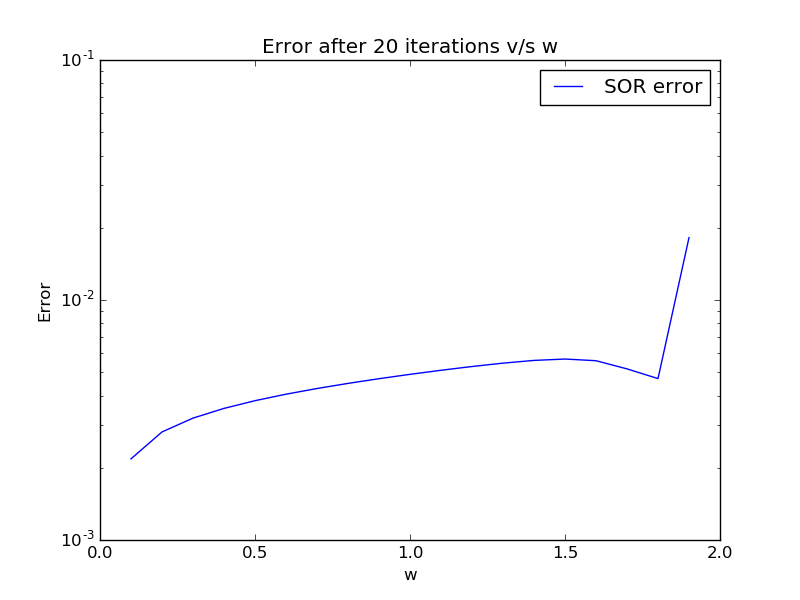
\includegraphics[width=0.8\textwidth]{nmax_20.png}
 \caption{Error v/s w for N = 20, nmax = 20}
\end{figure}

Note the though the minimum seems to occur at $w=0.1$, this is because of the definition of error used. (i.e we can see that
$\phi^{n+1} - \phi^{n} = w*\phi *$ so as w decreases the error decreases though it may not be near to the actual value). Thus
the optimum $w = 1.8$

The plots of the residues is shown below:
\begin{figure}[H]
 \centering
 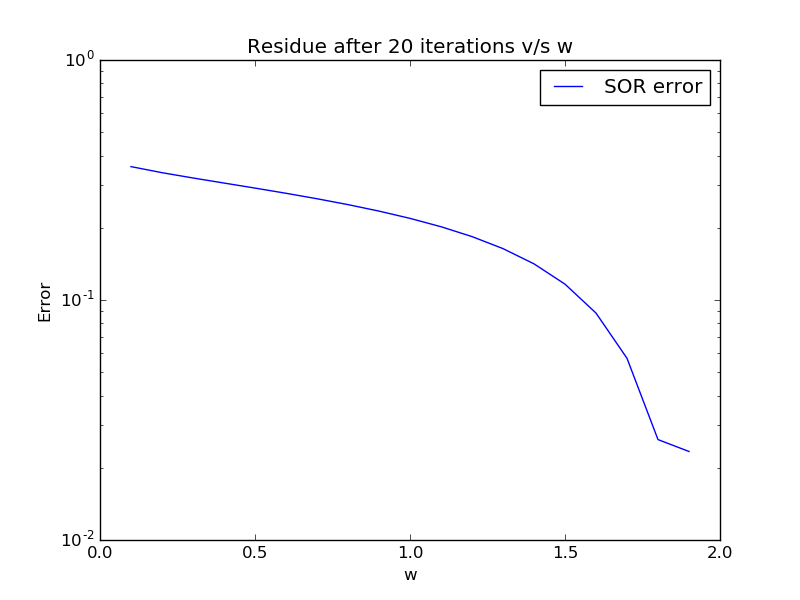
\includegraphics[width=0.8\textwidth]{nmax_20_1.png}
 \caption{Residue v/s w for N = 20, nmax = 20}
\end{figure}

We can see that in this case, the minimum occurs between $1.8$ and $w=1.9$. We can see that this plot gives a better visualization
of how changing $w$ affects the problem.


\section{Question 3:}
\label{Question3}
Here, we repeat the above question but for 50 and 100 iterations. The plot of final error v/s w for all three number of 
iterations is shown below
\begin{figure}[H]
 \centering
 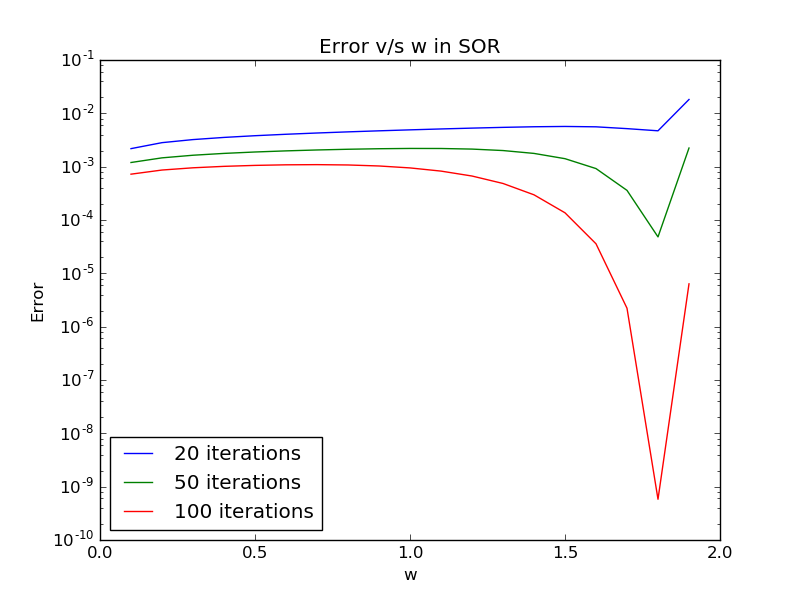
\includegraphics[width = 0.8\textwidth]{nmaxhigh.png}
 \caption{Final error v/s w for 20, 50 and 100 iterations}
\end{figure}

We can see that for all three iterations the minimum error occurs at $w=1.8$. This points to the fact that the optimum value
of $w$ doesn't depend on the number of iterations performed. But we do see that the error decreases as we increase the number
of iterations pointing to the fact that the scheme.

\section{Question 4:}
\label{Question4}
In this question, we are supposed to hunt a better value of $w$ tot he second decimal using 50 iterations. On plotting the graph
of error for w in the range $(1.7, 1.9)$, following graph is obtained
\begin{figure}[H]
 \centering
 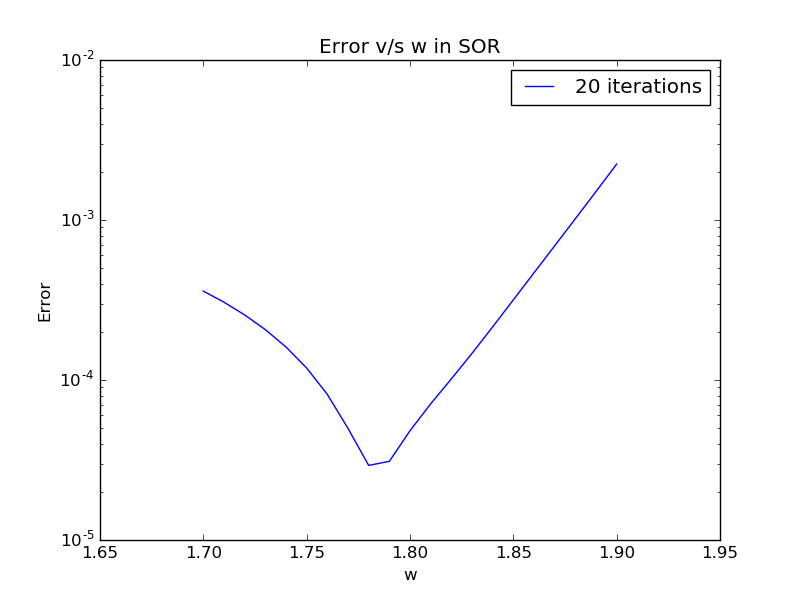
\includegraphics[width = 0.8\textwidth]{optw.png}
 \caption{Final error v/s w for 50 iterations}
\end{figure}

From the graph we can see that the optimum value for $w=1.78$


\section{Question 5:}
\label{Question5}
In this question, we repeat the above procedure for a grid size of $101$. We get the following graphs
\begin{figure}[H]
 \centering
 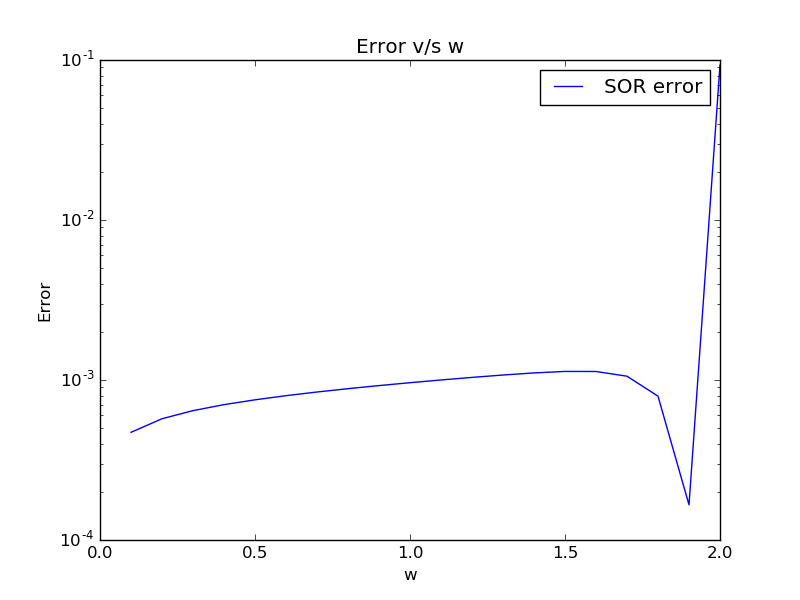
\includegraphics[width = 0.8\textwidth]{nmax_100_N_101.png}
 \caption{Final error v/s w for 100 iterations and 101 grid size}
\end{figure}
\begin{figure}[H]
 \centering
 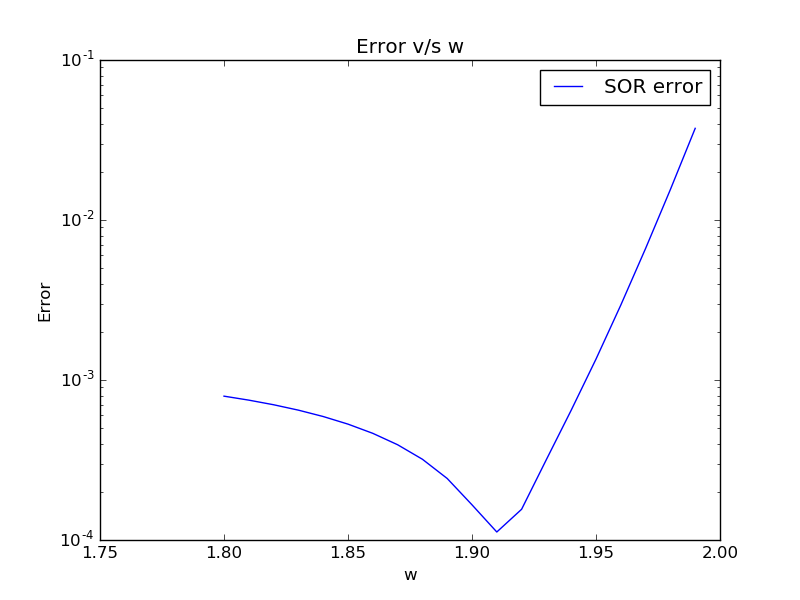
\includegraphics[width = 0.8\textwidth]{nmax_100_N_101_2.png}
 \caption{Final error v/s w for 100 iterations and 101 grid size}
\end{figure}

We see that the optimum $w = 1.91$ in this case, Thus optimum $w$ changes when the grid size changes.

\section{Question 6:}
\label{Question6}
In this question, we try to hunt for the optimum $w$ by letting the scheme converge to machine epsilon and checking the number
of iterations taken in the process. 
This is achieved by setting an arbitrarily high value of $nmax$ to ensure that the scheme converges before it reaches those
many iterations. The following graph is obtained:
\begin{figure}[H]
\centering
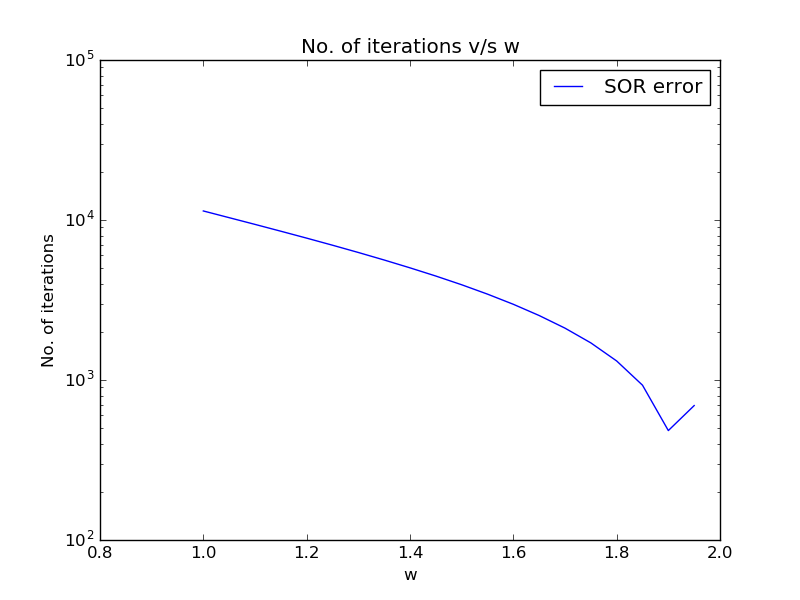
\includegraphics[width = 0.8\textwidth]{niter_w.png}
\end{figure}

We see this graph is similar to the previous graph and that the optimum $w = 1.91$

\section{Question 7:}
In this question we compare the convergence of the different schemes for grid size of 101. Following graph is obtained
\begin{figure}[H]
 \centering
 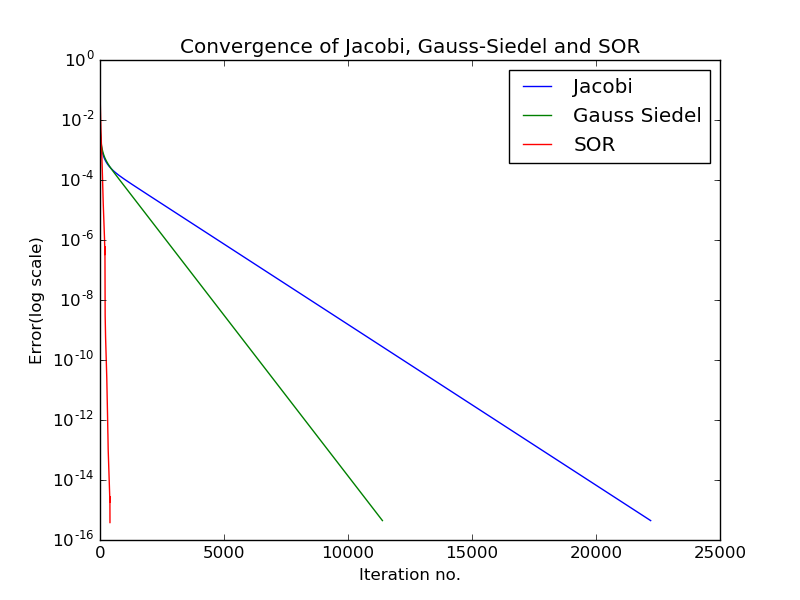
\includegraphics[width = 0.8\textwidth]{Comparison.png}
 \caption{Convergence of different schemes}
\end{figure}

From the graphs we can see that the Jacobi converges the slowest and SOR converges the fastest. We see that with the optimum value
of $w$, the SOR scheme improves convergence by orders of magnitude. Thus we can feel the power of the SOR scheme


\section{Conclusion}

This assignment gives us a better insight into the different schemes that can be used to solve Laplace equation (matrix equation
in general). We see that in case of Laplace equation Gauss Siedel is twice as fast as Jacobi scheme. We also learn how to
optimize the value of $w$ to achieve a better convergence rate. We see that this optimum value doesn't depend ont he number of 
iterations but only on the grid size. 

\end{document}

